\chapter{Introduction}

Large Language Models (LLMs) have rapidly evolved in recent years. These models, powered by deep learning techniques and vast datasets, are capable of understanding and generating human-like text with remarkable accuracy.

Modern and powerful natural language processing (NLP) models such as GPT-4 \cite{openai_gpt-4_2023} and Llama 3 \cite{dubey_llama_2024} are LLMs consisting of many transformer layers with billions of parameters. 

Despite their impressive performance across a diverse spectrum of tasks, these models' inherent complexity and scale pose significant challenges to understanding their inner workings and decision-making processes, thereby hindering their transparency and explainability. This causes these models to be understood as "black boxes" where they provide output to the user without providing any explanation or insight as to why this output was generated \cite{adadi_peeking_2018}. 

Unfortunately, the lack of effective interpretability of these models has hindered their deployment in critical domains such as healthcare, raising concerns around regulatory demands, safety, and ethical alignment \cite{goodman_european_2017, amodei_concrete_2016}. Furthermore, this opacity has restricted the use of LLMs in academic and data-driven fields \cite{ziems_can_2024}, where the priority is often to obtain a reliable interpretation rather than only to deploy the model. 

These problems have motivated the development of the field of Explainable AI (XAI) \cite{gilpin_explaining_2019} which focuses on creating methods to analyse the internal mechanisms of these models and provide explanations for their outputs.

One such technique for explainability is \emph{Counterfactual explanations} (CEs). A counterfactual explanation shows how an input, with the smallest change, can change the output of a classification model \cite{wachter_counterfactual_2017}.

\begin{figure}[h]
    \centering
    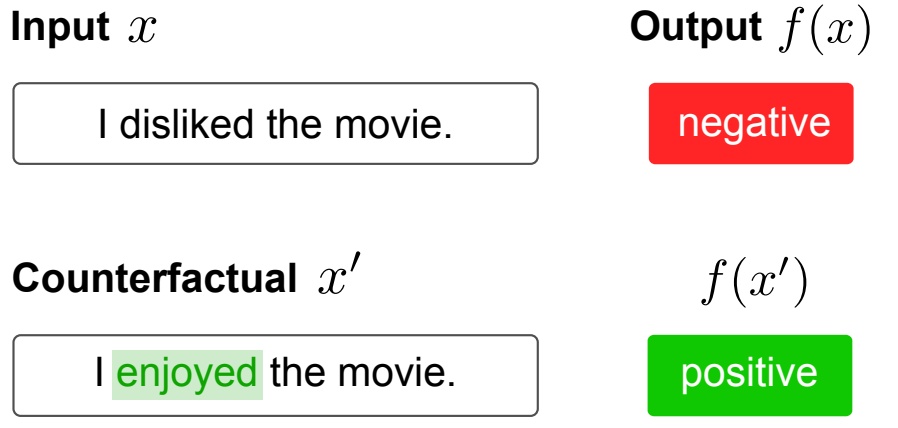
\includegraphics[width=0.55\textwidth]{counterfactual_intent_example.png}
    \caption{An example of a counterfactual explanation over sentiment \cite{mcaleese_comparative_2024}}
    \label{fig:enter-label}
\end{figure}

These allow us to explain and evaluate models and also augment training data \cite{kaushik_learning_2020}. Integrating augmented counterfactuals into training has shown an improvement in model performance over out-of-domain inputs \cite{kaushik_learning_2020, samory_call_2021}, which in turn helps models avoid unwanted generation due to inconsistencies in training data that may go unnoticed such as sexism \cite{sen_how_2021}

In the context of natural language processing, the generation of counterfactual explanations is not as straightforward as it is for tabular data as these counterfactual explanations should be close and comparable to the original text while still abiding by grammatical rules making a coherent sentence that is relevant. Guaranteeing validity is paramount for the deployment and trust of these models in high-precision and critical fields.

In the current landscape, there are white box methods that will generate word substitutions and construct counterfactuals \cite{pope_text_2021} by looking at internal model gradients, as well as black box methods such as prompting an LLM to generate counterfactuals \cite{wu_polyjuice_2021} leveraging the natural language generation and understanding pre-baked in LLMs to generate plausible counterfactuals. However, from benchmarks \cite{mcaleese_comparative_2024} we see that none of the existing methods are able to generate high-quality counterfactuals, as each method has some drawbacks with varying performance based on the context and dataset making them unreliable. White-box methods such as CLOSS generate mostly valid counterfactuals, however, they are frequently not plausible or realistic generations. However, LLM generation methods like FIZLE generate very correct and plausible counterfactuals but may modify the original input so much that it may stray from the original idea as well as not changing the output class making them invalid.

With new research in mechanistic interpretability techniques allowing for more robust and powerful ways to understand a model's inner workings \cite{ghandeharioun_patchscopes_2024}, we hope to propose a novel method that is able to expand on and combine the existing methods to generate high-quality counterfactual explanations with validity guarantees.